\documentclass[border=10pt]{standalone}

\usepackage{tikz}
\usepackage{tikzsymbols}
\usetikzlibrary{calc,patterns,shapes.geometric}

\def\centerarc[#1](#2)(#3:#4:#5){\draw[#1] ($(#2)+({#5*cos(#3)},{#5*sin(#3)})$) arc (#3:#4:#5);}

\begin{document}
	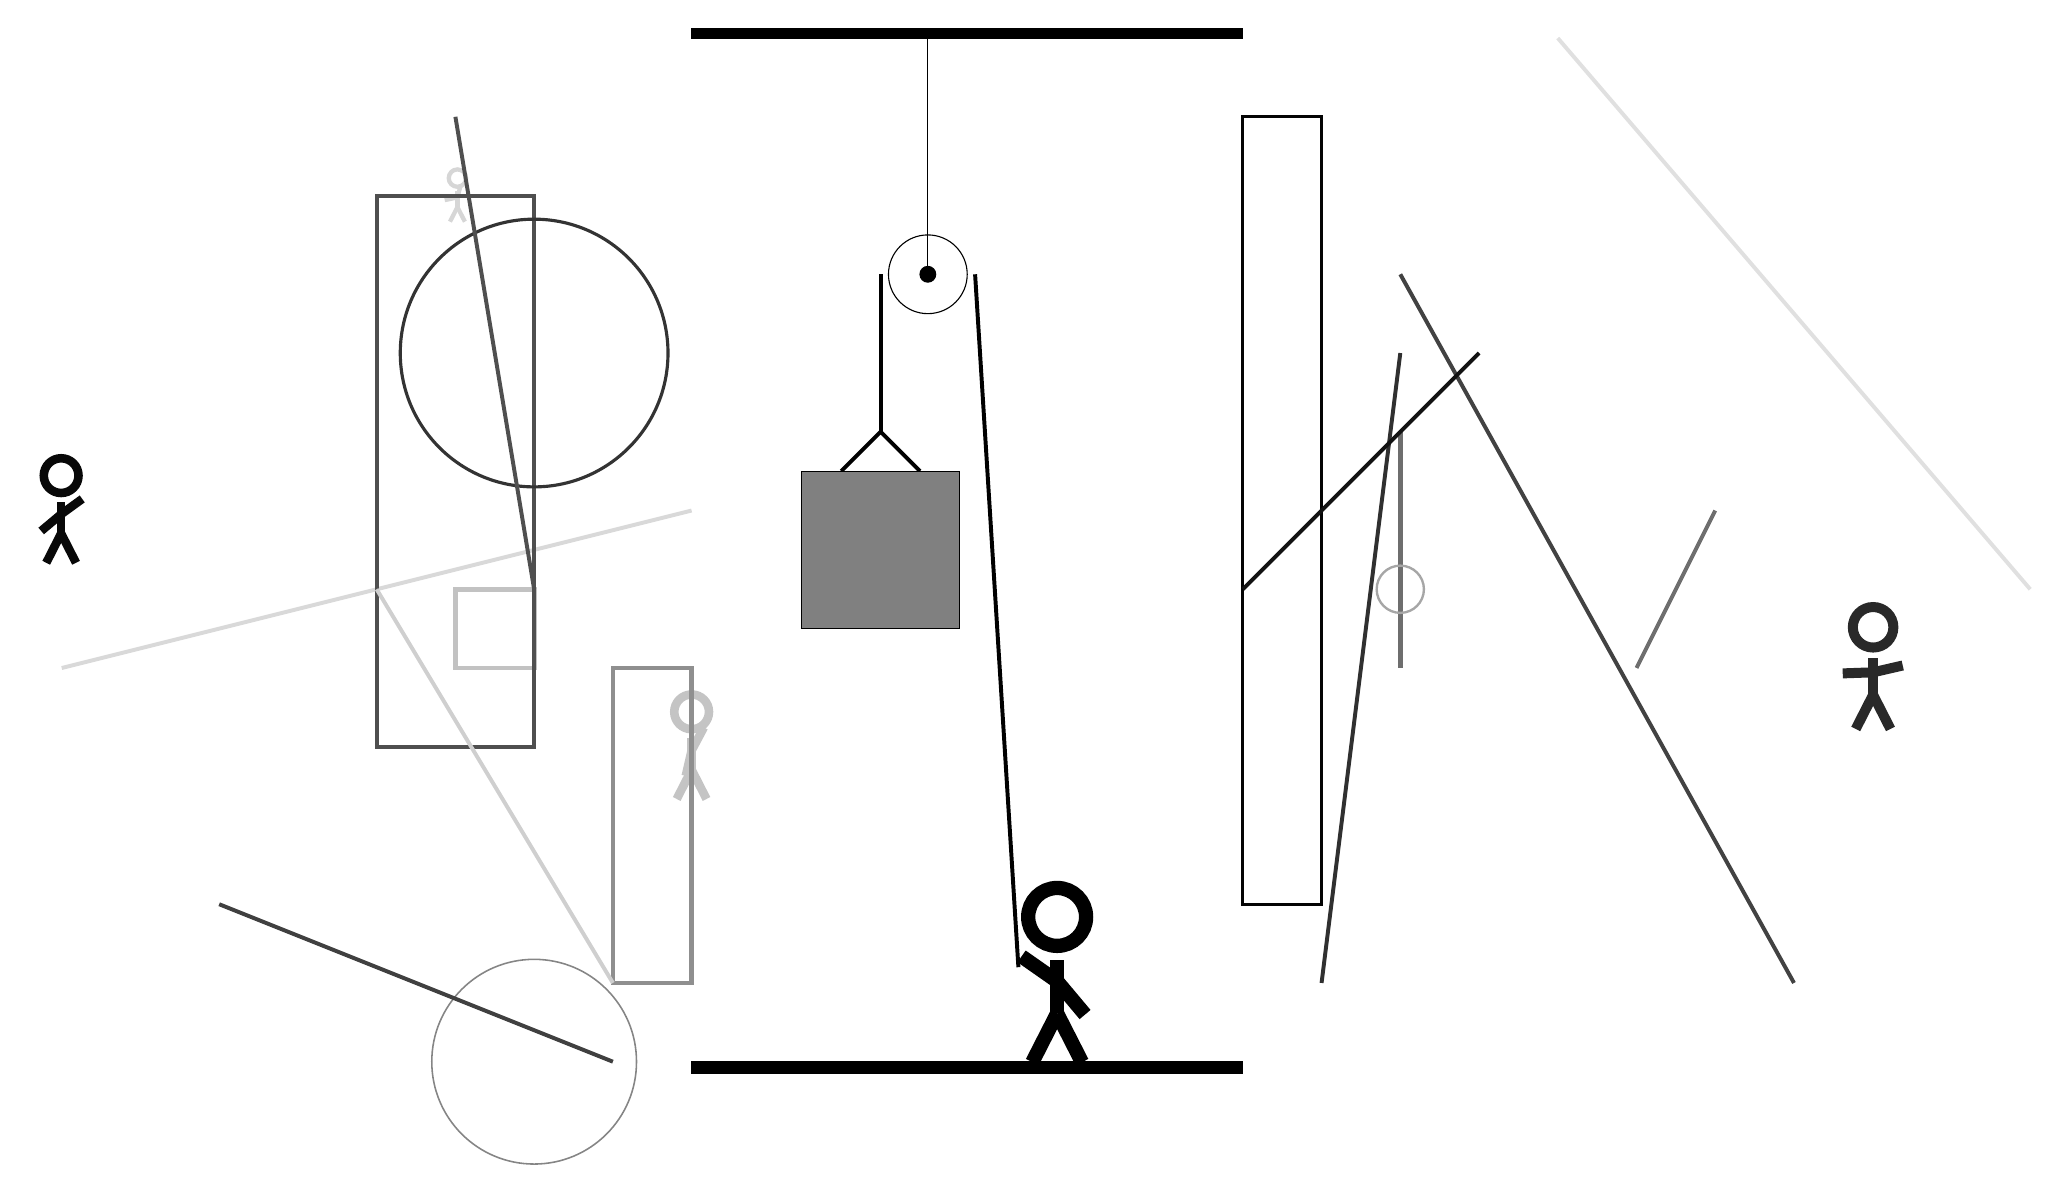
\begin{tikzpicture}
		%%%%% START %%%%%
		
		\draw[fill=black] (-2, 10) rectangle (5, 10.125);
		
		\draw (1, 7) circle (0.5);
		\draw[fill=black] (1, 7) circle (0.1);
		\draw (1, 10) -- (1, 7);
		
		\draw[line width=0.5mm] (-0.1, 4.5) -- (0.4, 5.0) -- (0.9, 4.5);
		\draw[fill=black!50] (-0.6, 4.5) rectangle (1.4, 2.5);
		
		\node[line width=0.5mm, color=black!23] at (-2, 1) {\Strichmaxerl[6][77][62]};
		
		\draw[line width=0.5mm, color=black!12](9, 10) -- (15, 3);
		\draw [line width=0.2mm, color=black!48](-4, -3) circle (1.3);
		\draw[line width=0.5mm, color=black!15](-2, 4) -- (-10, 2);
		
		\draw[line width=0.6mm, color=black!24] (-4, 3) rectangle (-5, 2);
		
		\draw[line width=0.5mm, color=black!57](10, 2) -- (11, 4);
		\node[line width=0.5mm, color=black!16] at (-5, 8) {\Strichmaxerl[3][12][75]};
		
		\draw[line width=0.5mm, color=black!75](-3, -3) -- (-8, -1);
		\draw[line width=0.4mm, color=black!99] (6, 9) rectangle (5, -1);
		\draw[line width=0.5mm, color=black!69] (-4, 8) rectangle (-6, 1);
		\node[line width=0.3mm, color=black!84] at (13, 2) {\Strichmaxerl[7][2][13]};
		
		\draw [line width=0.4mm, color=black!80](-4, 6) circle (1.7);
		\draw[line width=0.6mm, color=black!44] (-3, -2) rectangle (-2, 2);
		\draw[line width=0.5mm, color=black!69](-5, 9) -- (-4, 3);
		\draw[line width=0.5mm, color=black!81](7, 6) -- (6, -2);
		\draw[line width=0.6mm, color=black!57] (7, 2) rectangle (7, 5);
		
		\draw[line width=0.5mm, color=black!74](7, 7) -- (12, -2);
		\draw [line width=0.3mm, color=black!35](7, 3) circle (0.3);
		\draw[line width=0.5mm, color=black!93](8, 6) -- (5, 3);
		
		\draw[line width=0.5mm, color=black!19](-3, -2) -- (-6, 3);
		\node[line width=0.2mm, color=black!97] at (-10, 4) {\Strichmaxerl[6][40][36]};
		
		
		\draw[line width=0.5mm] (0.4, 7) -- (0.4, 5.0);
		\centerarc[line width=0.5mm](1, 7)(0:180:0.6);
		\draw[line width=0.5mm](1.6, 7) -- (2.15, -1.8);
		
		\node at (2.6, -1.9) {\Strichmaxerl[10][-35][-50]};
		
		\draw[fill=black] (-2, -3) rectangle (5, -3.15);
		
		%%%%% END %%%%%
	\end{tikzpicture}
\end{document}